\documentclass[english,a4paper,twoside]{report}

% Used packages
\usepackage[printonlyused]{acronym}
\usepackage[utf8]{inputenc}
\usepackage{amsfonts}
\usepackage{amsmath}
\usepackage{amssymb}
\usepackage{babel}
\usepackage{calc}
\usepackage{design}
\usepackage{fancyhdr}
\usepackage{graphicx}
\usepackage{tabularx}
\usepackage{listings}
\usepackage{url}

\newcommand{\AmbE}{Ambient~Earth}
\newcommand{\Amber}{\textsc{Amber}}

% Global settings.
\setlength{\parskip}{\medskipamount}
\setlength{\parindent}{0pt}

% Listing settings.
\lstset{basicstyle=\fontfamily{cmss}\small,frame=tb}
\lstset{columns=fixed,basewidth=0.5em,keepspaces=true}
\lstset{aboveskip=1em,belowskip=0.5em}
\lstset{numbers=left,numberstyle=\tiny,stepnumber=5}
\lstset{showtabs=false,showspaces=false,showstringspaces=false}

% Improved title page.
\makeatletter
\newcommand{\institution}{\newcommand{\@institution}}
\renewcommand\maketitle{\begin{titlepage}%
\let\footnotesize\small
\let\footnoterule\relax
\let \footnote \thanks
\null\vfil
\vskip 60\p@
\begin{center}%
  {\LARGE \@title \par}%
  \vskip 3em%
  {\large
   \lineskip .75em%
    \begin{tabular}[t]{c}%
      \@author
    \end{tabular}\par}%
    \vskip 1.5em%
  {\large \@date \par}%       % Set date in \large size.
\end{center}\par
\@thanks
\vfill
{\small
 \begin{flushright}
  \begin{tabular}{l}\hline
  \@institution\hline
  \end{tabular}
 \end{flushright}
}
\global\let\@institution\@empty
\global\let\institution\relax
\end{titlepage}
}

% Improved acronym environment.
\newenvironment{acronym*}[1]{%
   \newcommand{\acrolabel}[1]{\textbf{##1}\hfil}%
   \providecommand*{\acro}{\AC@acro}%
   \begin{list}{}{%
      \renewcommand{\makelabel}{\acrolabel}%
      \settowidth{\labelwidth}{\textbf{#1}}%
      \setlength{\leftmargin}{\labelwidth+\labelsep}%
      }
   }{%
   \end{list}
}\makeatother

% Fancy header settings.
\pagestyle{fancy}
\renewcommand{\chaptermark}[1]{\markboth{#1}{}}
\renewcommand{\sectionmark}[1]{\markright{\thesection\ #1}}
\fancyhf{}
\fancyheadoffset[LE,RO]{\marginparsep+\marginparwidth}
\fancyhead[LE,RO]{\bfseries\thepage}
\fancyhead[LO]{\bfseries\rightmark}
\fancyhead[RE]{\bfseries\leftmark}
\fancypagestyle{plain}{%
  \fancyhead{}\renewcommand{\headrulewidth}{0pt}}

% Document meta data.
%FIXME: better title & remove draft suffix
\title{Ambient Earth\\
       {\Large \emph{Design Document --- 1$^{\text{st}}$ draft\/}}}
\author{Christian Luijten\\\url{christian06@ru.is}}
\date{\today}
\institution{
 CADIA group \\
 School of Science and Engineering \\
 Reykjavík University, Reykjavík \\[1em]
 \emph{Under supervision of:\/} \\
 Kristinn R. Thórisson, Ph.D. (Reykjavík University) \\
 dr.ir. Huub van de Wetering (Eindhoven University of Technology) \\
}

% Macros.
\newcommand{\anode}[1]{\textsl{#1\/}}
\newcommand{\atype}[1]{\ensuremath{\textsl{#1\/}}}
\newcommand{\content}[1]{\textsl{#1\/}}
\newcommand{\entry}[1]{\texttt{#1}}
\renewcommand{\implies}{\Rightarrow}
\newcommand{\pole}{\addtocounter{fd@flagcount}{1}}
\newcommand{\mblstinline}[1]{\mbox{[\lstinline[columns=fixed]{#1}]}}
\newcommand{\q}{\quad}
\newcommand{\strtok}[1]{\textbf{`#1'}}

\begin{document}

\acrodef{RU}{Reykjavík University}
\acrodef{CADIA}{Center for Analysis \& Design of Intelligent Agents}
\acrodef{RSS}{Rich Site Summary}

\maketitle

% \abstract{
  % Ambient Earth is a software system for analysis of Internet activity. This
  % document describes the design of the system.
 % }

\tableofcontents

\chapter{Introduction}

This document describes the design of the \AmbE\ project. The ambitional goal
of this project is to give an ambient view on the activity on the whole
world-wide web. In practice, it shows the activity on for instance a forum or
larger weblog system.

The design of the project will follow the Constructionist Design Methodology
for Interactive Intelligences\cite{CDM}. First, a few usage scenarios are given
in Chapter~\ref{cpt:scenarios}. Then in Chapter~\ref{cpt:requirements}
requirements are summed up. Using the requirements, an architecture is written
up in Chapter~\ref{cpt:architecture}.


\include{design-scenarios.inc}

\chapter{\label{cpt:requirements}Requirements}

There are various kinds of requirements to be identified. A distinction can be
made between functional and extra-functional (or non-functional) requirements.

\section{Extra-functional requirements}

\begin{enumerate}
  \item The system must make use of the Psyclone framework for communication.
  \item The system will be implemented in the Java programming language.
  \item The display module with the Java Applet must be able to run on any
        machine with the Java plugins properly installed (i.e. not only on the
        machine running the rest of the system).
  \item It must be possible to add modules with similar functionality to
        operate in parallel with modules already there. For example when the
        Java Applet is running, it should also be possible to have the full
        screen module running at the same time. 
\end{enumerate}

\section{Functional requirements}

These requirements describe which \emph{inputs}, \emph{outputs}, \emph{storage}
and \emph{computations} exist in the system and how they are \emph{timed and
synchronized}.

\subsection{Inputs}

\begin{enumerate}
  \item The system must be configurable to specify which RSS feeds will be
        monitored.
  \item The configuration of the system does not have to be done during run-time.
  \item Changing the configuration of a module may require a restart of the
        module.
  \item The system will use the configuration to get information from the
        internet from the specified RSS feeds.
  \item The display may have a set of controls to navigate through the history
        of a feed.
  \item Parts of the system must accept triggers from Psyclone whiteboards.
\end{enumerate}

\subsection{Outputs}

\begin{enumerate}
  \item There will be an output module which is to be used within a website, i.e. a Java Applet.
  \item There will be an output module which can display more information than
        the Applet which runs in full screen.
\end{enumerate}

\subsection{Storage}

\begin{enumerate}
  \item The system on itself does not store anything.
\end{enumerate}

\subsection{Computations}

\begin{enumerate}
  \item The system must decide of a delivered story what its subject(s) is/are.
  \item The system may put weights on the subjects instead of a boolean value.
\end{enumerate}

\subsection{Timing and synchronization}

\begin{enumerate}
  \item Synchronization between modules is handled by Psyclone, so no
        requirements need to be added to the system itself.
\end{enumerate}



\chapter{Architecture}

\chapter[Components]{Components of \AmbE}


\section{Crawler}

\subsection{RSS}


\section{Parser}

\subsection{Keywords}

\subsection{Phrases}


\section{Display}

\subsection{Full screen}

\subsection{Ambient applet}



\section{\label{sct:messages}Messages}


\subsection{Between Crawler and Sieve}


\subsection{Between Sieve and ShowOff}






\chapter{Detailed design}

In this chapter, every single class is described in terms of interface and
functionality. Because of the fairly dynamic character of this project -- new
ideas come and go -- this chapter will not be finished until the end of the
project and will probably change regularly.

\section{Files and directories}

All source code will be in the directory \texttt{src/}. All classes are in the
package \texttt{amber} or in a subpackage thereof. The Psyclone specification
file \texttt{psySpec.xml} is found in \texttt{data/}. External libraries that
are redistributed with \Amber\ are in \texttt{lib/}. The source of this
document, the traineeship report and the website are located in
\texttt{documentation/}.

The application is built using Apache
Ant\footnote{\url{http://ant.apache.org/}} and it can be imported into
Eclipse\footnote{\url{http://www.eclipse.org/}}. It requires Java SDK version
1.5 or greater.

\section{Crawler module}

\begin{figure}
  \centering
  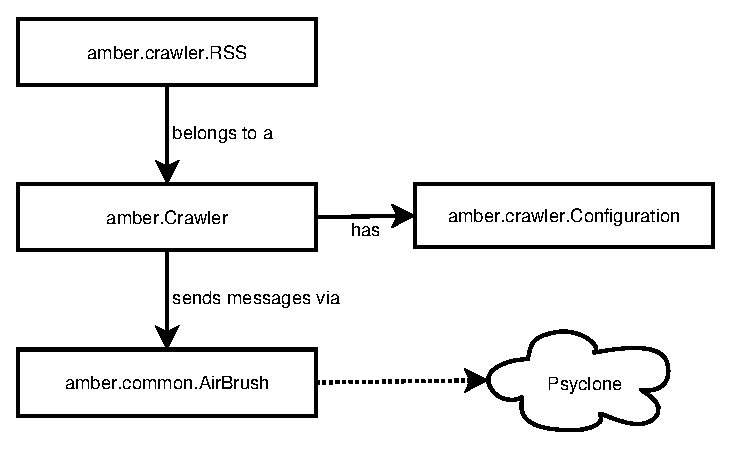
\includegraphics{image/crawler}
  \caption{
    Diagram of the design of the Crawler, the names are Java classnames
  }
\end{figure}


\section{Sieve module}

\section{ShowOff module}

\begin{figure}
  \centering
  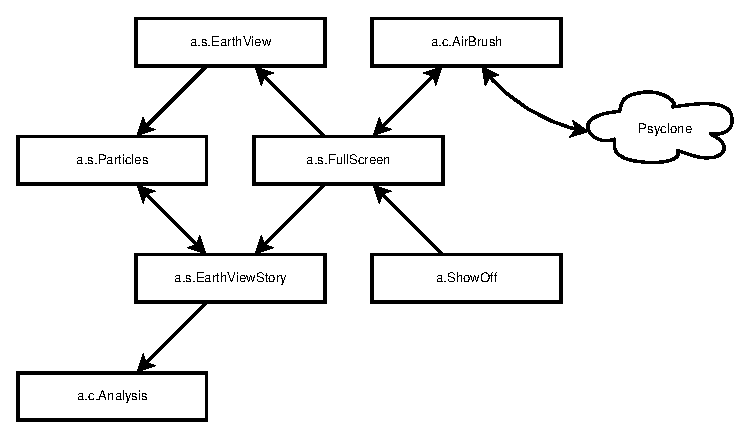
\includegraphics{image/showoff-fullscreen}
  \caption{
    Diagram of the design of the full screen ShowOff module, the names are
    abbreviated Java classnames
  }
\end{figure}



% \include{design-conclusion.inc}

% \appendix

\bibliographystyle{cadia}
\bibliography{bibliography}
\addcontentsline{toc}{chapter}{\refname}

\end{document}
